
\documentclass{report}
\usepackage[utf8]{inputenc}
\usepackage[T1]{fontenc}
\usepackage{anysize} 
\usepackage{siunitx}
\usepackage{longtable,fancyhdr}
\usepackage{amsmath}
\usepackage{amsfonts}
\usepackage{amssymb}
\usepackage{listings}
\usepackage[dvipsnames,usenames,table,xcdraw]{xcolor}
\usepackage{booktabs}
\usepackage{caption}
\usepackage{mdframed}
\usepackage{float}
\usepackage{subcaption}
\usepackage[nogin]{Sweave}
\usepackage{lscape}
\usepackage{pdfpages}
\usepackage{xcolor} % Required for colour specification
\usepackage[linktocpage]{hyperref}
\usepackage{titlesec}
\usepackage{fancyvrb}
\usepackage{rotating} 

\marginsize{1.0cm}{2.25cm}{1.0cm}{1.0cm}

\setlength{\topmargin}{-0.5cm}
\setlength{\textheight}{23cm}
\setlength{\textwidth}{16cm}
\setlength{\oddsidemargin}{0.5cm}

\setlength{\abovedisplayskip}{0pt}
\setlength{\belowdisplayskip}{0pt}
\setlength{\abovedisplayshortskip}{0pt}
\setlength{\belowdisplayshortskip}{0pt}

\renewcommand{\baselinestretch}{1.1}
\renewcommand{\topfraction}{0.99}
\renewcommand{\bottomfraction}{0.99}
\renewcommand{\familydefault}{\sfdefault}
\renewcommand{\arraystretch}{1.5}
\renewcommand{\chaptername}{Partie}
\newcommand{\plogo}{\fbox{$\mathcal{PL}$}} % Generic dummy publisher logo
\renewcommand{\chaptername}{Part}

\DeclareMathOperator*{\argmaxA}{arg\,max} %

\titleformat{\chapter}[display]
{\normalfont\bfseries}{}{0pt}{\Huge}

\titlespacing*{\chapter}{0pt}{-50pt}{40pt}

\addtocontents{toc}{\protect\thispagestyle{empty}}

\mdfsetup{frametitlealignment=\center}

\def\Y{{\rm Y}}
\def\var{\hbox{var}}
\def\npde{{\rm npde}}
\def\pde{{\rm pde}}
\def\npd{{\rm npd}}
\def\pd{{\rm pd}}
\def\vec{{\rm vec}}
\def\ypred{{\rm ypred}}
\def\R{{\sf R}}
\def\true{{\sf TRUE}}
\def\false{{\sf FALSE}}

\definecolor{codegreen}{rgb}{0,0.6,0}
\definecolor{codegray}{rgb}{0.5,0.5,0.5}
\definecolor{codepurple}{rgb}{0.58,0,0.82}
\definecolor{backcolour}{rgb}{0.95,0.95,0.92}

% background code chunk listing
\lstdefinestyle{mystyle}{
%basicstyle=\ttfamily\footnotesize,
xleftmargin=3.4pt,
xrightmargin=3.4pt,
backgroundcolor=\color{backcolour},   
commentstyle=\color{codegreen},
keywordstyle=\color{magenta},
numberstyle=\tiny\color{white},
stringstyle=\color{codepurple},
basicstyle=\small\ttfamily,
breakatwhitespace=false,         
breaklines=true, 
rulecolor=\color{black},
captionpos=t,                    
keepspaces=true,    
frame=single,
language=R,
numbers=left,                    
%numbersep=5pt,       
showspaces=false,                
showstringspaces=false,
showtabs=false,                  
tabsize=2,
aboveskip  = 1.0\baselineskip, 
belowskip = 1.0\baselineskip
}

\lstset{style=mystyle}

\begin{document}

\thispagestyle{empty}

\Sconcordance{concordance:BeautifulGraphs-Npde-v3.tex:BeautifulGraphs-Npde-v3.Rnw:%
1 130 1 1 9 57 1 1 43 1 11 12 1 1 3 2 0 1 3 1 0 1 3 1 %
0 1 2 3 0 1 2 2 1 1 2 46 0 1 1 41 0 1 1 53 0 1 1 43 0 %
1 2 31 1 1 2 4 0 1 2 220 1 1 2 4 0 1 2 6 1 2 2 2 1 1 %
2 4 0 1 2 6 1 2 2 2 1 1 2 4 0 1 2 6 1 2 2 2 1 1 2 4 0 %
1 2 6 1 2 2 2 1 1 2 4 0 1 2 6 1 2 2 6 1 1 2 4 0 1 2 5 %
1 2 2 2 1 1 2 4 0 1 2 5 1 2 2 6 1 1 2 1 0 1 1 3 0 1 2 %
5 1 2 2 6 1 2 2 6 1 1 2 1 0 1 1 3 0 1 2 5 1 2 2 5 1 2 %
2 2 1 1 2 4 0 1 2 5 1 2 2 10 1 1 2 4 0 1 2 6 1 2 2 2 %
1 1 34 36 0 1 2 6 1 1 34 1 2 18 1 1 57 59 0 1 2 7 1 1 %
56 1 2 2 1 1 2 4 0 1 2 6 1 2 2 2 1 1 2 4 0 1 2 6 1 1 %
3 1 2 6 1 1 2 1 0 2 1 3 0 1 2 5 1 1 4 1 2 6 1 1 2 1 0 %
1 1 3 0 1 2 6 1 2 2 5 1 2 2 6 1 1 3 5 0 1 2 6 1 1 3 1 %
2 2 1 1 5 7 0 1 2 6 1 1 4 1 2 2 1 1 53 55 0 1 2 6 1 1 %
56 1 2 4 1}


%\SweaveOpts{prefix.string=FiguresUserGuide/Fig}

\pagestyle{fancy}
\renewcommand{\headrulewidth}{0pt}
\renewcommand{\footrulewidth}{1pt}
\renewcommand{\thesection}{\arabic{section}}
%\renewcommand{\footrulewidth}{0pt}
\lhead{}
\chead{}
\rhead{}
\lfoot{\itshape NPDE group, \today}
\cfoot{User guide for the NPDE library.}
\rfoot{\thepage}

% Indenting
\DefineVerbatimEnvironment{Sinput}{Verbatim}{xleftmargin=2em,fontshape=sl,fontfamily=tt}
\DefineVerbatimEnvironment{Soutput}{Verbatim}{xleftmargin=2em,fontshape=sl,fontfamily=tt}
\DefineVerbatimEnvironment{Scode}{Verbatim}{xleftmargin=2em,fontshape=sl,fontfamily=tt}
\fvset{listparameters={\setlength{\topsep}{-1pt}}}
\renewenvironment{Schunk}{\vspace{\topsep}}{\vspace{\topsep}}

\parindent 18pt
$\phantom{minime}$

\begin{figure}[htp] 
\captionsetup[subfigure]{labelformat=empty}

\centering
\subfloat[]{%
\includegraphics[scale=0.8]{ParisDiderotLogo.png}%
}%
\hfill%
\subfloat[]{%
\includegraphics[scale=0.5]{InsermLogo.png}%
}%
\end{figure}


\begin{center}
{\setlength{\baselineskip}{2\baselineskip}
{\Large \bfseries Beautiful graphs with npde 3.0}

\parindent 18pt
$\phantom{minime}$

{\Large \bfseries F\'evrier 2021}

\bigskip

{\Large \itshape \bfseries Emmanuelle Comets, Romain Leroux}

\bigskip

\bigskip

{\large \itshape \bfseries Contributors to npde: Karl Brendel, Marc Cerou, Romain Leroux, Thi Huyen Tram Nguyen, France Mentr\'e}

\bigskip
{\it
INSERM, IAME UMR 1137, Paris, France

Universit\'e de Paris, Paris, France.
}
\par}
\end{center}

\vskip 2.5cm
\begin{center}
\large \bfseries{Npde website}:\url{www.npde.biostat.fr}
\end{center}

\newpage

\tableofcontents

\newpage

% Loading libraries:


\setcounter{page}{1}

%********************************************************************************************************************
\section{Running npde }
%********************************************************************************************************************

% Describe:
% - viral load data 
% - theophyline
% - warfarine

\begin{lstlisting}[linerange=\\begin\{Sinput\}-\\end\{Sinput\}, includerangemarker=false]
\begin{Schunk}
\begin{Sinput}
> # virload20
> yvir20 <- autonpde(virload20,simvirload,iid=1,ix=2,iy=3, icens=4, boolsave=FALSE)
> # theopp
> theofit1 <- autonpde(theopp,simtheopp,1,3,4,boolsave=FALSE, units=list(x="hr",y="mg/L"))
> # warfarine
> wbase<-autonpde(namobs=warfarin,namsim=simwarfarinBase, iid=1,ix=2,iy=4,icov=c(3,6:8),namsav="warfBase", units=list(x="hr",y="ug/L", covariates=c("mg","kg","-","yr")))
> wcov<-autonpde(namobs=warfarin,namsim=simwarfarinCov, iid=1,ix=2,iy=4,icov=c(3,6:8),namsav="warfCov", units=list(x="hr",y="ug/L", covariates=c("mg","kg","-","yr")))
\end{Sinput}
\end{Schunk}
\end{lstlisting}

\begin{mdframed}[backgroundcolor=green!13]
\begin{Schunk}
\begin{Sinput}
> yvir20
\end{Sinput}
\begin{Soutput}
Object of class NpdeObject
-----------------------------------------
----        Component data           ----
-----------------------------------------
Object of class NpdeData
    Structured data: Log_VL ~ Time | ID 
This object has the following components:
     data: data
     with 50 subjects
      300 observations
The data has the following components
     X: Time () 
     Y: Log_VL () 
     individual model predictions: ipred 
     missing data: mdv  (1=missing)
     censored data: cens  (1=censored)
      LOQ:     1.3 
-----------------------------------------
----        Component results        ----
-----------------------------------------
Object of class NpdeRes
  containing the following elements:
    predictions (ypred)
    prediction discrepancies (pd)
    normalised prediction distribution errors (npde)
    completed responses (ycomp) for censored data
    decorrelated responses (ydobs)
    ploq: probability of being <LOQ for each observation
  the dataframe has  300 non-missing observations .
First 10 lines of results, removing missing observations:
       ypred ycomp    pd        npde       ydobs     tnpde
1  4.4099809  3.95 0.307 -0.50437199 -0.50389104 1.4356698
2  2.4975561  1.91 0.229 -0.55923698 -0.57968771 1.3609386
3  1.9229180  1.89 0.493  1.11232137  1.03971370 3.6377559
4  1.6290177  1.69 0.538  0.37454350  0.39208593 2.6328341
5  1.3697648  1.63 0.640  0.48736457  0.47523309 2.7865068
6  0.8601327  1.55 0.821  1.19011804  0.95569947 3.7437222
7  4.3566026  4.42 0.534  0.08532879  0.06968412 2.2388969
8  2.4636655  2.55 0.579  0.06521854  0.09265785 2.2115048
9  1.9063313  1.48 0.265 -1.35317415 -1.37472078 0.2795226
10 1.6029737  1.48 0.424  0.78236516  0.66459383 3.1883250
\end{Soutput}
\begin{Sinput}
> theofit1
\end{Sinput}
\begin{Soutput}
Object of class NpdeObject
-----------------------------------------
----        Component data           ----
-----------------------------------------
Object of class NpdeData
    Structured data: Conc ~ Time | ID 
This object has the following components:
     data: data
     with 12 subjects
      120 observations
The data has the following components
     X: Time (hr) 
     Y: Conc (mg/L) 
     missing data: mdv  (1=missing)
-----------------------------------------
----        Component results        ----
-----------------------------------------
Object of class NpdeRes
  containing the following elements:
    predictions (ypred)
    prediction discrepancies (pd)
    normalised prediction distribution errors (npde)
    completed responses (ycomp) for censored data
    decorrelated responses (ydobs)
  the dataframe has  120 non-missing observations and 132 lines.
First 10 lines of results, removing missing observations:
      ypred ycomp    pd       ydobs      npde     tnpde
2  2.923864  2.84 0.550 -0.05124648 0.1256613  5.403817
3  4.682299  6.57 0.850  1.96398150 2.0537489 11.302178
4  6.264357 10.50 0.990  2.56602650 2.3263479 12.136107
5  6.986255  9.66 0.980  0.41616411 0.5244005  6.623631
6  6.511039  8.58 0.930  0.28430866 0.2533471  5.794430
7  5.895675  8.36 0.960  0.54879386 0.6744898  7.082780
8  5.064736  7.47 0.970  1.79335938 1.6448536 10.051295
9  4.302909  6.89 0.990  0.80506269 0.7721932  7.381673
10 3.294020  5.94 0.995  1.91537662 1.7506861 10.375055
11 1.168743  3.28 0.995  3.25535923 2.5758293 12.899315
\end{Soutput}
\begin{Sinput}
> wbase
\end{Sinput}
\begin{Soutput}
Object of class NpdeObject
-----------------------------------------
----        Component data           ----
-----------------------------------------
Object of class NpdeData
    Structured data: dv ~ time | id 
    Covariates: amt wt sex 
This object has the following components:
     data: data
     with 32 subjects
      247 observations
The data has the following components
     X: time (hr) 
     Y: dv (ug/L) 
     missing data: mdv  (1=missing)
-----------------------------------------
----        Component results        ----
-----------------------------------------
Object of class NpdeRes
  containing the following elements:
    predictions (ypred)
    prediction discrepancies (pd)
    normalised prediction distribution errors (npde)
    completed responses (ycomp) for censored data
    decorrelated responses (ydobs)
  the dataframe has  247 non-missing observations .
First 10 lines of results, removing missing observations:
        ypred ycomp    pd       ydobs       npde
1   0.5814627   0.0 0.359 -0.43862113 -0.3611330
2   3.1220995   1.9 0.454 -0.05116685  0.1636585
3   8.4386880   3.3 0.126 -1.35607837 -1.4985131
4  11.2936700   6.6 0.140  0.04661369  0.1560419
5  12.6249280   9.1 0.127 -0.56691520 -0.5417366
6  11.7504645  10.8 0.355  0.89677342  0.9230138
7  10.8386881   8.6 0.141 -1.08057832 -1.1358962
8   8.5881834   5.6 0.026 -1.89143682 -1.8521799
9   7.0369975   4.0 0.019 -1.06275059 -1.0278933
10  5.7174611   2.7 0.017 -0.60300349 -0.5947658
         tnpde
1   4.79538371
2   6.98209215
3   0.05613313
4   6.95035522
5   4.04284249
6  10.14618430
7   1.56708994
8  -1.41753046
9   2.01711779
10  3.82187933
\end{Soutput}
\begin{Sinput}
> wcov
\end{Sinput}
\begin{Soutput}
Object of class NpdeObject
-----------------------------------------
----        Component data           ----
-----------------------------------------
Object of class NpdeData
    Structured data: dv ~ time | id 
    Covariates: amt wt sex 
This object has the following components:
     data: data
     with 32 subjects
      247 observations
The data has the following components
     X: time (hr) 
     Y: dv (ug/L) 
     missing data: mdv  (1=missing)
-----------------------------------------
----        Component results        ----
-----------------------------------------
Object of class NpdeRes
  containing the following elements:
    predictions (ypred)
    prediction discrepancies (pd)
    normalised prediction distribution errors (npde)
    completed responses (ycomp) for censored data
    decorrelated responses (ydobs)
  the dataframe has  247 non-missing observations .
First 10 lines of results, removing missing observations:
        ypred ycomp    pd       ydobs       npde      tnpde
1   0.3746216   0.0 0.398 -0.34893746 -0.2585273  5.2792639
2   2.6728119   1.9 0.500 -0.03334944  0.1535051  6.8242576
3   8.0288884   3.3 0.115 -1.43486957 -1.5300676  0.5113814
4  10.9755216   6.6 0.106 -0.32327872 -0.2845355  5.1817410
5  12.2572079   9.1 0.063 -0.96158402 -0.9944579  2.5197520
6  11.3470900  10.8 0.381  0.71955362  0.7421442  9.0314719
7  10.4732161   8.6 0.107 -1.05944210 -1.0581216  2.2810327
8   8.0557699   5.6 0.026 -1.82921396 -1.9268366 -0.9763794
9   6.3939722   4.0 0.030 -0.99871382 -0.9862713  2.5504491
10  5.0984787   2.7 0.026 -0.69323563 -0.6588377  3.7782238
\end{Soutput}
\end{Schunk}
\end{mdframed}

%********************************************************************************************************************
\section{Types of graphs}
%********************************************************************************************************************

\hskip 18pt Each of the default diagnostic plots, as well as a number of additional plots not shown by default, can also be produced on its own, using the argument \verb+plot.type="type"+. Table~\ref{tab:plottypes} lists the plots that can be created in this way. 

\begin{table}[!h]
%\noindent{\bfseries Table II:} {\itshape Types of plots available.}
%\label{tab:plot.types}
\begin{center}
\begin{tabular} {| r p{10cm} |}
\hline {\bf Plot type} & {\bf Description} \\
\hline
data & Plots the observed data in the dataset \\
hist & Histogram of the \npde \\
qqplot & QQ-plot of the \npde versus its theoretical distribution  \\
ecdf & Empirical distribution function of the \npde\\
x.scatter & Scatterplot of the \npde~versus the predictor X \\
pred.scatter & Scatterplot of the \npde~versus the population predicted values \\
cov.scatter & Scatterplot of the \npde~versus covariates \\
vpc & Plots a Visual Predictive Check (VPC) \\
loq & Plots the probability for an observation to be BQL, versus the predictor X \\
\hline
\end{tabular}
\end{center}
\caption{Plot types available in the {\sf npde} library. QQ-plots, histograms, cumulative cdf, and scatter plots can be produced for \npde, \pd~or \npd.} \label{tab:plottypes}
\end{table}

\noindent This function for plotting is:
\begin{lstlisting}[linerange=\\begin\{Sinput\}-\\end\{Sinput\}, includerangemarker=false]
\begin{Schunk}
\begin{Sinput}
> plot(x,plot.type="data")
\end{Sinput}
\end{Schunk}
\end{lstlisting} 

\noindent The first argument, x, is a {\sf NpdeObject} and plot.type argument is used to specify the type of graph.

%********************************************************************************************************************
\section{Changing graphical parameters}
%********************************************************************************************************************

Default layout for graphs in the npde library can be modified through the use of many options. An additional document, demo npde2.0.pdf, is included in the inst directory of the package, presenting additional examples of graphs and how to change the options. 
Tables \nameref{tab:graphicalOptions1},\nameref{tab:graphicalOptions2}
\nameref{tab:graphicalOptions3},\nameref{tab:graphicalOptions4},\nameref{tab:graphicalOptions5}, following table shows the options that can be set, either by specifying them on the fly in a call to plot applied to a NpdeObject object, or by storing them in the prefs component of the object. Note that not all of the graphical parameters in
par() can be used, but it is possible for instance to use the xaxt="n" option below to suppress plotting
of the X-axis, and to then add back the axis with the R function axis() to tailor the tickmarks or change
colours as wanted. It is also possible of course to extract npde, fitted values or original data to produce any of these plots by hand if the flexibility provided in the library isn’t sufficient. 

\begin{table}[!h] 
\begin{center}
\begin{tabular}{| r p{8cm} c|}
\hline
\textbf{\textcolor{black}{Argument}} & \centering{\textbf{\textcolor{black}{Description }}} & \textbf{\textcolor{black}{Default value}} \\
\hline
{\ttfamily verbose} & Output is produced for some plots (most notably when binning is used, this prints out the boundaries of the binning intervals) if TRUE & FALSE \\
{\ttfamily main} & Title & depends on plot \\
{\ttfamily sub } & Subtitle & empty \\
{\ttfamily size.main } & Size of the main title & 14 \\
{\ttfamily size.sub  } & Size of the title for covariate & 12 \\

{\ttfamily xlab} & Label for the X-axis & depends on plot \\
{\ttfamily ylab} & Label for the Y-axis & depends on plot \\
{\ttfamily size.xlab} & Size of the label for the X-axis & 12 \\
{\ttfamily size.ylab} & Size of the label for the Y-axis & 12 \\
{\ttfamily breaks.x} & Number of tick marks on the X-axis & 10 \\
{\ttfamily breaks.y} & Number of tick marks on the Y-axis & 10 \\
{\ttfamily size.x.text} & Size of tick marks and tick labels on the X-axis & 10 \\
{\ttfamily size.y.text} & Size of tick marks and tick labels on the Y-axis & 10 \\

{\ttfamily xlim} & Range of values on the X-axis & empty, adjusts to the data \\
{\ttfamily ylim} & Range of values on the Y-axis & empty, adjusts to the data \\

{\ttfamily xaxt} & A character whether to plot the X axis. Specifying "n" suppresses plotting of the axis & "y"  \\
{\ttfamily yaxt} & A character whether to plot the Y axis. Specifying "n" suppresses plotting of the axis & "y" \\

{\ttfamily xlog} & Scale for the X-axis (TRUE: logarithmic scale) & FALSE \\
{\ttfamily ylog} & Scale for the Y-axis (TRUE: logarithmic scale) & FALSE \\

{\ttfamily } & &  \\
\hline
\end{tabular} 
\end{center}
\caption{Graphical parameters that can be passed on the plot function: titles and axes.} \label{tab:graphicalOptions1}
\end{table} 

\clearpage

\begin{table}[!h] 
\vspace{-2cm}
\begin{center}
\begin{tabular}{| r p{8cm} c|}
\hline
\textbf{\textcolor{black}{Argument}} & \centering{\textbf{\textcolor{black}{Description }}} & \textbf{\textcolor{black}{Default value}} \\
\hline
{\ttfamily col} & Main colour for observed data (applied to lines and symbols pertaining to observations if no other option is given to supersede this value) & "slategray4"  \\
{\ttfamily lty} & Line type for observed data & 1 \\
{\ttfamily lwd} & Line width for observed data & 0.5 \\
{\ttfamily pch} & Symbol used to plot observed data &  20 \\
{\ttfamily alpha} & Transparencyfor observed data  & 1 \\
{\ttfamily size} & Symbol size to plot observed data & 1  \\
{\ttfamily fill} & Colour used to fill area elements related to observed data (such as histogram bars) & "white  \\
{\ttfamily } & &  \\

{\ttfamily fill.outliers.med} & Color for the outliers of the median confidence interval & "red"  \\
{\ttfamily fill.outliers.bands} & Color for the outliers of  the bounds of the confidence interval & "red"  \\
{\ttfamily alpha.outliers.med} & Transparency of the color for the outliers of the median confidence interval & 1  \\
{\ttfamily alpha.outliers.bands} & Transparency of the color  for the outliers the bounds of the confidence interval & 1  \\
{\ttfamily } & &  \\

{\ttfamily col.bands} &  Colour for the lines of the bounds of the confidence interval & "steelblue4"  \\
{\ttfamily lty.bands} &  Type for the lines of bounds
of the confidence interval & 2  \\
{\ttfamily lwd.bands} &  Width of the lines of bounds
of the confidence interva & 0.25  \\
{\ttfamily alpha.bands} &  Transparency of the bounds of the confidence interval & "0.3"  \\
{\ttfamily fill.bands} &  Colour of the confidence interval & "steelblue2"  \\
{\ttfamily } & &  \\
{\ttfamily col.med} &  Colour for the lines of the median of the confidence interval & "salmon4"  \\
{\ttfamily lty.med} &  Type for the lines of the median
of the confidence interval & 2  \\
{\ttfamily lwd.med} &  Width of the lines of the median
of the confidence interva & 0.5  \\
{\ttfamily alpha.med} &  Transparency of of the median confidence interval & "0.5"  \\
{\ttfamily fill.med} &  Colour of the median confidence  interval & "pink"  \\
{\ttfamily } & &  \\

{\ttfamily type } &  Type for the line for qqplot and scatter. Display line and points. & "b"  \\
\hline
\end{tabular} 
\end{center}
\caption{Graphical parameters that can be passed on the plot function: colours and symbols.} \label{tab:graphicalOptions2}
\end{table} 

\clearpage

\begin{table}[!h] 
\begin{center}
\begin{tabular}{| r p{8cm} c|}
\hline
\textbf{\textcolor{black}{Argument}} & \centering{\textbf{\textcolor{black}{Description }}} & \textbf{\textcolor{black}{Default value}} \\
\hline
{\ttfamily col.pobs} & Colour for observed data & "slategray4"  \\
{\ttfamily pch.pobs} & Symbol used to plot observed data &  20 \\
{\ttfamily size.pobs} & Symbol size to plot observed data & 1.5  \\
{\ttfamily alpha.pobs} & Transparencyfor observed data  & 1.5 \\
{\ttfamily } & &  \\

{\ttfamily col.lobs} & Colour for the line of observed data & "slategray4"  \\
{\ttfamily lty.lobs} & Line type for the line of observed data &  20 \\
{\ttfamily lwd.lobs} & Line width  for the line of observed data & 1.5  \\
{\ttfamily } & &  \\

{\ttfamily col.pcens} & Colour for the censored data  & "red"  \\
{\ttfamily pch.pcens} & Symbol for the censored data  &  8 \\
{\ttfamily size.pcens} & Symbol size for the censored data  &  1.2 \\
{\ttfamily alpha.pcens} &Transparency for the censored data & 1  \\
{\ttfamily } & &  \\

{\ttfamily col.line.loq} & Colour for the LOQ line  & "black"  \\
{\ttfamily lty.line.loq} & Symbol type for the LOQ line &  5 \\
{\ttfamily lwd.line.loq} & Symbol size for the LOQ line &  0.5 \\
{\ttfamily } & &  \\

\hline
\end{tabular} 
\end{center}
\caption{Graphical parameters that can be passed on the plot function: colours and symbols.} \label{tab:graphicalOptions3}
\end{table} 


\begin{table}[H] 
\begin{center}
\begin{tabular}{|r p{10cm} p{3cm} |}
\arrayrulecolor{black}\hline
& \centering {\textbf{\textcolor{black}{Graphical options for VPC and residual plots}}} & \\
\centering{\textbf{\textcolor{black}{Parameter}} }& \centering{\textbf{\textcolor{black}{Description }}} & \textbf{\textcolor{black}{Default value}} \\
\hline
{\ttfamily bands} & Whether prediction intervals should be plotted & TRUE \\
{\ttfamily approx.pi} & If TRUE, samples from $\mathcal{N}(0,1)$ are used to plot prediction intervals, while if FALSE, prediction bands are obtained using pd/npde computed for the simulated data & TRUE \\
{\sf bin.method} & Method used to bin points (one of "equal", "width", "user" or "optimal"); at least the first two letters of the method need to be specified & "equal" \\
{\ttfamily bin.number} & Number of binning intervals & 10 \\
{\ttfamily vpc.interval} & Size of interval & 0.95 \\
{\ttfamily bin.breaks} & Vector of breaks used with user-defined breaks (vpc.method="user") & NULL \\
{\ttfamily bin.extreme} & Can be set to a vector of 2 values to fine-tune the behaviour of the binning algorithm at the boundaries; specifying c(0.01,0.99) with the "equal" binning method and vpc.bin=10 will create 2 extreme bands containing 1\% of the data on the X-interval, then divide the region within the two bands into the remaining 8 intervals each containing the same number of data; in this case the intervals will all be equal except for the two extreme intervals, the size of which is fixed by the user; complete fine-tuning can be obtained by setting the breaks with the vpc.method="user" & NULL \\
{\ttfamily pi.size} & Width of the prediction interval on the quantiles & 0.95 \\
{\ttfamily bin.lambda} & Value of lambda used to select the optimal number of bins through a penalised criterion & 0.3 \\
{\ttfamily bin.beta} & Value of beta used to compute the variance-based criterion (Jopt,beta(I)) in the clustering algorithm & 0.2 \\
{\ttfamily bands.rep} & Number of simulated datasets used to compute prediction bands & 200 \\
\hline
\end{tabular} 
\end{center}
\caption{Graphical options for VPC and residual plots.} \label{tab:graphicalOptions4}
\end{table} 

\clearpage

\begin{table}[!h] 
\begin{center}
\begin{tabular}{| r p{8cm} c|}
\hline
\textbf{\textcolor{black}{Argument}} & \centering{\textbf{\textcolor{black}{Description }}} & \textbf{\textcolor{black}{Default value}} \\
\hline
 {\ttfamily plot.box } & If TRUE, boxplots are produced instead of scatterplots & FALSE \\
 {\ttfamily covsplit } & If TRUE, plot are split by covariates & FALSE \\
 {\ttfamily plot.loq } & If TRUE, data under the LOQ are plotted & FALSE \\
 {\ttfamily line.loq } & If TRUE, horizontal line should is plotted at Y=LOQ in data and VPC plots & FALSE \\
 {\ttfamily impute.loq } & If TRUE, the imputed values are plotted for data under the LOQ & FALSE \\
% {\ttfamily bands } & If TRUE, prediction bands should be added to the plots & TRUE \\
 {\ttfamily plot.obs } & If TRUE, observations, pd/ndpe should are plotted on top of the prediction bands & TRUE \\
 {\ttfamily grid } & If TRUE, display a grid on the background of the plot & FALSE \\
 {\ttfamily box } & If TRUE, boxplots are be performed instead of scatterplots (see documentation) & FALSE \\
{\ttfamily } & &  \\

\hline
\end{tabular} 
\end{center}
\caption{Boolean parameters that can be passed on the plot function.} \label{tab:graphicalOptions5}
\end{table} 








%********************************************************************************************************************
\section{Default plots}
%********************************************************************************************************************

%********************************************************************************************************************
\subsection{Waffle plot}
%********************************************************************************************************************
By default, the package produces and saves the four graphs:

\begin{itemize}
\item[1.] a quantile-quantile plot: plot of the npde versus the corresponding quantiles of a normal distribution
\begin{itemize}
\item[$\bullet$] the line y = x is also drawn
\end{itemize}
\item[2.] a histogram of the npde
\begin{itemize}
\item[$\bullet$] the shape of the normal distribution $\mathcal{N}$(0,1) is also shown
\end{itemize}
\item[3.] a plot of the npde versus the independent variable X
\item[4.] a plot of the npde versus ypred
\begin{itemize}
\item[$\bullet$]  for these last two graphs, we plot the lines corresponding to y = 0 and to the critical values
5\% and 95\% (delimiting the 90\% confidence interval in which we expect to nd the bulk of
the npde).
\end{itemize}
\end{itemize}

\begin{lstlisting}[linerange=\\begin\{Sinput\}-\\end\{Sinput\}, includerangemarker=false]
\begin{Schunk}
\begin{Sinput}
> plot(yvir20)
\end{Sinput}
\end{Schunk}
\end{lstlisting}


\begin{figure}[H]
\caption{Default plot for yvir20.}
\label{fig:plotByDefault}
\centering
\includegraphics{BeautifulGraphs-Npde-v3-008}
\end{figure}

\begin{lstlisting}[linerange=\\begin\{Sinput\}-\\end\{Sinput\}, includerangemarker=false]
\begin{Schunk}
\begin{Sinput}
> plot(theofit1)
\end{Sinput}
\end{Schunk}
\end{lstlisting}


\begin{figure}[H]
\caption{Default plot for theofit1.}
\label{fig:plotByDefault}
\centering
\includegraphics{BeautifulGraphs-Npde-v3-010}
\end{figure}

\begin{lstlisting}[linerange=\\begin\{Sinput\}-\\end\{Sinput\}, includerangemarker=false]
\begin{Schunk}
\begin{Sinput}
> plot(wbase)
\end{Sinput}
\end{Schunk}
\end{lstlisting}


\begin{figure}[H]
\caption{Default plot for wbase.}
\label{fig:plotByDefault}
\centering
\includegraphics{BeautifulGraphs-Npde-v3-012}
\end{figure}

\begin{lstlisting}[linerange=\\begin\{Sinput\}-\\end\{Sinput\}, includerangemarker=false]
\begin{Schunk}
\begin{Sinput}
> plot(wcov)
\end{Sinput}
\end{Schunk}
\end{lstlisting}


\begin{figure}[H]
\caption{Default plot for wcov.}
\label{fig:plotByDefault}
\centering
\includegraphics{BeautifulGraphs-Npde-v3-014}
\end{figure}

\begin{lstlisting}[linerange=\\begin\{Sinput\}-\\end\{Sinput\}, includerangemarker=false]
\begin{Schunk}
\begin{Sinput}
> plot(theofit1,col.pobs="green",pch.pobs=3,size.pobs=2)
\end{Sinput}
\end{Schunk}
\end{lstlisting}


\begin{figure}[H]
\caption{Default plot for theofit1 with user defined options for the observations.}
\label{fig:plotByDefault}
\centering
\includegraphics{BeautifulGraphs-Npde-v3-016}
\end{figure}

%********************************************************************************************************************
\subsection{Data}
%********************************************************************************************************************

\begin{lstlisting}[linerange=\\begin\{Sinput\}-\\end\{Sinput\}, includerangemarker=false]
\begin{Schunk}
\begin{Sinput}
> plot(theofit1,plot.type="data")
\end{Sinput}
\end{Schunk}
\end{lstlisting}

\begin{figure}[H]
\caption{Default plot for theofit1 - data.}
\label{fig:plotByDefault}
\centering
\includegraphics{BeautifulGraphs-Npde-v3-018}
\end{figure}

\begin{lstlisting}[linerange=\\begin\{Sinput\}-\\end\{Sinput\}, includerangemarker=false]
\begin{Schunk}
\begin{Sinput}
> plot(yvir20,plot.type="data",plot.loq=TRUE,line.loq=TRUE)
\end{Sinput}
\end{Schunk}
\end{lstlisting}

\begin{figure}[H]
\caption{Default plot for yvir20 - data.}
%\label{}
\centering
\includegraphics{BeautifulGraphs-Npde-v3-020}
\end{figure}

%********************************************************************************************************************
\subsection{VPC (Visual Predictive Check)}
%********************************************************************************************************************

\begin{lstlisting}[linerange=\\begin\{Sinput\}-\\end\{Sinput\}, includerangemarker=false]
\begin{Schunk}
\begin{Sinput}
> plot(theofit1,plot.type="vpc")
> plot(theofit1, plot.type="vpc", plot.box=TRUE)
\end{Sinput}
\end{Schunk}
\end{lstlisting}

\begin{figure}[H]
\caption{Default plot for theofit1 - VPC.}
\label{fig:plotByDefault}
\centering
\includegraphics{BeautifulGraphs-Npde-v3-022}
\end{figure}


\begin{figure}[H]
\caption{Default plot for theofit1 with boxplots.}
\label{fig:plotByDefault}
\centering
\includegraphics{BeautifulGraphs-Npde-v3-023}
\end{figure}

%********************************************************************************************************************
\subsection{Scatterplots: scatterplots of npde versus X or predictions}
%********************************************************************************************************************

\begin{lstlisting}[linerange=\\begin\{Sinput\}-\\end\{Sinput\}, includerangemarker=false]
\begin{Schunk}
\begin{Sinput}
> plot(theofit1,plot.type="x.scatter")
> plot(theofit1,plot.type="pred.scatter")
\end{Sinput}
\end{Schunk}
\end{lstlisting}

\begin{figure}[H]
\caption{Default plot for theofit1 - scatterplot of npde vs X.}
\label{fig:plotByDefault}
\centering
\includegraphics{BeautifulGraphs-Npde-v3-025}
\end{figure}

\begin{figure}[H]
\caption{Default plot for theofit1 - scatterplot of npde vs predictions.}
\label{fig:plotByDefault}
\centering
\includegraphics{BeautifulGraphs-Npde-v3-026}
\end{figure}

\begin{lstlisting}[linerange=\\begin\{Sinput\}-\\end\{Sinput\}, includerangemarker=false]
\begin{Schunk}
\begin{Sinput}
> plot(yvir20 , plot.type="x.scatter", plot.box=TRUE)
\end{Sinput}
\end{Schunk}
\end{lstlisting}

\begin{figure}[H]
\caption{Default plot for theofit1 - scatterplot of npde vs X with boxplot.}
\label{fig:plotByDefault}
\centering
\includegraphics{BeautifulGraphs-Npde-v3-028}
\end{figure}

%********************************************************************************************************************
\section{Histogram, QQ-plot and Ecdf plots.}
%********************************************************************************************************************

%********************************************************************************************************************
\subsection{Histogram}
%********************************************************************************************************************

\begin{lstlisting}[linerange=\\begin\{Sinput\}-\\end\{Sinput\}, includerangemarker=false]
\begin{Schunk}
\begin{Sinput}
> plot(yvir20,plot.type="hist")
\end{Sinput}
\end{Schunk}
\end{lstlisting}


\begin{figure}[H]
\caption{Histogram plot for yvir20.}
\label{fig:Histogram_plot01_yvir20}
\centering
\includegraphics{BeautifulGraphs-Npde-v3-030}
\end{figure}

\begin{lstlisting}[linerange=\\begin\{Sinput\}-\\end\{Sinput\}, includerangemarker=false]
\begin{Schunk}
\begin{Sinput}
> plot(yvir20,plot.type="hist",which="npde",
      main = "Title",
      size.main = 14,
      sub = "",
      size.sub = "",
      xlab= "Sample quantiles (npde)",
      ylab= "Frequency",
      size.xlab = 12, ## cex.axis = 12
      size.ylab = 12,
      #xlim=c(0,25),
      #ylim=c(-3,3.5),
      xlim=c(),
      ylim=c(),
      bands=TRUE, # TRUE, FALSE
      lty.grid="dotted",
      col = "green",
      fill = "skyblue",
      alpha = 0.95,
      lty = 2,
      lwd = 1,
      col.bands = "red",
      fill.bands = "red" ,
      alpha.bands = 0.5,
      lty.bands = 1,
      lwd.bands = 0.5,
      col.pobs = "darkblue",
      size.pobs = 2,
      size.text.x = 10,
      size.text.y = 10,
      breaks.x = 10,
      breaks.y = 10,
      xlog = FALSE,
      ylog = FALSE)
\end{Sinput}
\end{Schunk}
\end{lstlisting} 


\begin{figure}[H]
\caption{Histogram plot for yvir20 with user defined options.}
\label{fig:Histogram_plot01_yvir20}
\centering
\includegraphics{BeautifulGraphs-Npde-v3-032}
\end{figure}

%********************************************************************************************************************
\subsection{QQ-plot}
%********************************************************************************************************************

%********************************************************************************************************************
\subsection{Ecdf plots}
%********************************************************************************************************************

%********************************************************************************************************************
\section{x.scatter and pred.scatter plots}
%********************************************************************************************************************

%********************************************************************************************************************
\subsection{x.scatter plots}
%********************************************************************************************************************

\begin{lstlisting}[linerange=\\begin\{Sinput\}-\\end\{Sinput\}, includerangemarker=false]
\begin{Schunk}
\begin{Sinput}
> plot(theofit1, plot.type="x.scatter",
      
      main = "npde vs time data xtheo_cens",
      size.main = 14,
      sub = "",
      size.sub = "",
      
      xlab= "Time",
      ylab= "pd",
      size.xlab = 12, ## cex.axis = 12
      size.ylab = 12,
      #xlim=c(0,25),
      #ylim=c(-3,3.5),
      xlim=c(),
      ylim=c(),
      
      approx.pi=TRUE,
      bands=TRUE,
      plot.obs=TRUE,
      
      alpha.med = 0.25,
      fill.med = "firebrick4",
      col.med="red",
      lty.med=3,
      lwd.med=1,
      
      alpha.bands = 0.25,
      fill.bands = "dodgerblue",
      col.bands="green",
      lty.bands=6,
      lwd.bands=1,
      
      col.med = "red",
      lty.med = 1,
      lwd.med = 1,
      
      col.bands = "blue",
      lty.bands = 1,
      lwd.bands = 1,
      
      col.pobs = "orangered3",
      pch.pobs = 12,
      size.pobs = 1.5,
      
      col.pcens = "yellow",
      pch.pcens = 15,
      size.pcens = 1.75,
      
      size.text.x = 10,
      size.text.y = 10,
      
      breaks.x = 1,
      breaks.y = 10,
      
      xlog = FALSE,
      ylog = FALSE)
\end{Sinput}
\end{Schunk}
\end{lstlisting}



\begin{figure}[H]
\caption{x.scatter plot for the theofit1 with user defined options}
%\label{}
\centering
\includegraphics{BeautifulGraphs-Npde-v3-034}
\end{figure}

\begin{lstlisting}[linerange=\\begin\{Sinput\}-\\end\{Sinput\}, includerangemarker=false]
\begin{Schunk}
\begin{Sinput}
> plot(yvir20, plot.type="x.scatter", plot.box=TRUE)
\end{Sinput}
\end{Schunk}
\end{lstlisting}


\begin{figure}[H]
\caption{x.scatter plot for the theofit1 with boxplots}
%\label{}
\centering
\includegraphics{BeautifulGraphs-Npde-v3-036}
\end{figure}

\begin{lstlisting}[linerange=\\begin\{Sinput\}-\\end\{Sinput\}, includerangemarker=false]
\begin{Schunk}
\begin{Sinput}
> plot(wcov, plot.type="x.scatter", covsplit=TRUE, which.cov=c("sex","wt"))
\end{Sinput}
\end{Schunk}
\end{lstlisting}


\begin{figure}[H]
\caption{Wcov data - npde versus X, split according to sex and wt}
%\label{}
\centering
\includegraphics{BeautifulGraphs-Npde-v3-038}
\end{figure}

%********************************************************************************************************************
\section{Waffle plot}
%********************************************************************************************************************

\begin{lstlisting}[linerange=\\begin\{Sinput\}-\\end\{Sinput\}, includerangemarker=false]
\begin{Schunk}
\begin{Sinput}
> plot.x.scatter.yvir20 = plot(yvir20,plot.type="x.scatter")
> plot.pred.scatter.yvir20 = plot(yvir20,plot.type="pred.scatter")
> do.call(grid.arrange, c(plot.x.scatter.yvir20, plot.pred.scatter.yvir20, list( nrow=1, ncol=2)))
\end{Sinput}
\end{Schunk}
\end{lstlisting}


\begin{figure}[H]
\caption{yvir20 data - Waffle plot}
\centering
\includegraphics{BeautifulGraphs-Npde-v3-040}
\end{figure}

%********************************************************************************************************************
\section{Plot LOQ}
%********************************************************************************************************************

\begin{lstlisting}[linerange=\\begin\{Sinput\}-\\end\{Sinput\}, includerangemarker=false]
\begin{Schunk}
\begin{Sinput}
> plot(yvir20, plot.type="loq")
> plot(yvir20, plot.type="loq", lwd.bands=1.75)
\end{Sinput}
\end{Schunk}
\end{lstlisting}


\begin{figure}[H]
\caption{Default plots - fraction of data below LOQ.}
%\label{}
\centering
\includegraphics{BeautifulGraphs-Npde-v3-042}
\end{figure}

\begin{figure}[H]
\caption{Default plots - fraction of data below LOQ, with user defined options.}
%\label{}
\centering
\includegraphics{BeautifulGraphs-Npde-v3-043}
\end{figure}

%********************************************************************************************************************
\section{Options for plots}
%********************************************************************************************************************

\begin{lstlisting}[linerange=\\begin\{Sinput\}-\\end\{Sinput\}, includerangemarker=false]
\begin{Schunk}
\begin{Sinput}
> plot(yvir20,plot.type="data",main="Raw data",
 col.pobs="DarkRed",col.lobs="DarkRed", col.pcens="blue", pch.pobs=2,pch.pcens=20,lty.lobs=2,xlab="The X-axis", ylab="The Y-axis",sub="Some changes",cex=0.8, cex.lab=1.5, plot.loq=TRUE)
\end{Sinput}
\end{Schunk}
\end{lstlisting}


\begin{figure}[H]
\caption{Plots - options for data.}
%\label{}
\centering
\includegraphics{BeautifulGraphs-Npde-v3-045}
\end{figure}

\begin{lstlisting}[linerange=\\begin\{Sinput\}-\\end\{Sinput\}, includerangemarker=false]
\begin{Schunk}
\begin{Sinput}
> plot(yvir20,plot.type="ecdf",main="yvir20",col.pobs="DarkRed",col.lobs="DarkRed",
 col.pcens="blue",pch.pobs=2,pch.pcens=20,lty.lobs=2,xlab="The X-axis",
 ylab="The Y-axis",sub="Some changes",cex=0.8, cex.lab=1.5,bands=TRUE,
 col.fillpi="lightgreen",col.lpi="green")
\end{Sinput}
\end{Schunk}
\end{lstlisting}


\begin{figure}[H]
\caption{Plots - options for ecdf.}
%\label{}
\centering
\includegraphics{BeautifulGraphs-Npde-v3-047}
\end{figure}

\begin{lstlisting}[linerange=\\begin\{Sinput\}-\\end\{Sinput\}, includerangemarker=false]
\begin{Schunk}
\begin{Sinput}
> plot(yvir20,plot.type="vpc",
      main = "yvir20 vpc",
      size.main = 14,
      sub = "",
      size.sub = "",
 
      xlab="The X-axis",
      ylab="The Y-axis",
      
      size.xlab = 12, ## cex.axis = 12
      size.ylab = 12,
 
      bands=TRUE,
      plot.obs=TRUE,
 
      col.line.loq = "orange",
      lty.line.loq  = 4,
      lwd.line.loq  = 1,
 
      alpha.med = 0.25,
      fill.med = "firebrick4",
      col.med="red",
      lty.med=3,
      lwd.med=1,
 
      alpha.bands = 0.25,
      fill.bands = "dodgerblue",
      col.bands="green",
      lty.bands=6,
      lwd.bands=1,
 
      col.med = "red",
      lty.med = 1,
      lwd.med = 1,
 
      col.bands = "blue",
      lty.bands = 1,
      lwd.bands = 1,
 
      col.pobs = "orangered3",
      pch.pobs = 12,
      size.pobs = 1.5,
 
      col.pcens = "yellow",
      pch.pcens = 15,
      size.pcens = 1.75,
 
      size.text.x = 10,
      size.text.y = 10,
 
      breaks.x = 10,
      breaks.y = 10)
\end{Sinput}
\end{Schunk}
\end{lstlisting}


\begin{figure}[H]
\caption{Plots - options for VPC.}
%\label{}
\centering
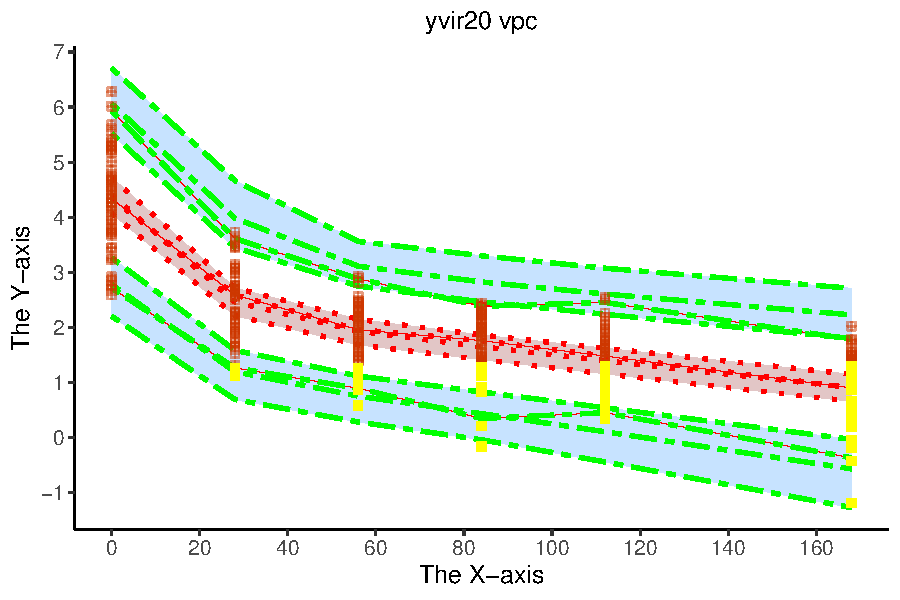
\includegraphics{BeautifulGraphs-Npde-v3-049}
\end{figure}
     
     

\end{document}
